% !TEX root = ../EjercPracticas.tex

\formatoEjecicio

%\falta{Hay que tener en cuenta que esta relación puede durar unas 3 semanas. A la cuarta semana está el parcial (sesión 8). También podemos dedicar dos semanas y dejar la tercera semana para resolver dudas tanto de estas relaciones como de los ejercicios propuestos. Tendremos que planificarlo muy bien.}



Independientemente de la lista siguiente de ejercicios,  transformar en función o funciones \underline{\bf \large todos} los  ejercicios que ya has resuelto en las relaciones anteriores.  Procura usar siempre la mayor cantidad de funciones posibles. Recuerda que una función tiene un propósito específico (resuelve un problema) y como para cada ejercicio tuviste, en su caso, que descomponer el problema en subproblemas deberías, como mínimo, tener una función por cada subproblema. Si dicho subproblema se descompusiera en subsubproblemas, resuélvelo invocando a las funciones asociadas a los subsubproblemas.
 
 


\begin{ejercicio}
Construya con PyCharm una estructura de directorios para implementar el juego de \textit{Piedra, Papel y Tijera} para repasar la programación estructurada y modular.

\begin{pyverbatim}[][frame=single]
import random
...
if __name__ == '__main__':
    turnos = 3
    run(turnos)
\end{pyverbatim}

\end{ejercicio}

\begin{quote}
El juego consiste en dos jugadores que ocultan sus manos y al contar tres cada uno saca una de las manos con una postura concreta. Hay 3 posturas de las mano: la de piedra, la de papel y la de tijera. Unas posturas ganan a otras. Cada vez que la postura de la mano de un jugador gana a la postura del otro jugador, el primero gana un punto. El proceso finaliza hasta que uno de los jugadores tenga más puntos que la mitad de los turnos que se haya establecido previamente. Por ejemplo, si el número de turnos es 3 entonces la partida gana el mejor de 3 (el que consiga 2 puntos), si el número de turnos es 4 entonces la partida finaliza al mejor de 3 (el que consiga 3 puntos). Finalizada la partida los jugadores pueden abandonar o echar otra partida con el mismo número de turnos.

Un turno es el proceso por el que los dos jugadores sacan sus manos, comparan las posiciones y asignan un punto más o ninguno a cada uno de ellos de acuerdo a la siguiente tabla de beneficios:

\centerline{\begin{tabular}{|c|ccc|}\hline
\textbf{Beneficios} & Piedra & Papel & Tijera \\ \hline
Piedra & (0,0)  & (0,1) & (1,0)  \\
Papel  & (1,0)  & (0,0) & (0,1)  \\
Tijera & (0,1)  & (1,0) & (0,0) \\ \hline
\end{tabular}}

En nuestra versión del juego, un jugador será el ordenador y el otro jugador será un humano. Durante un turno, el humano puede decidir abandonar la partida. En el caso de terminar la partida, recuerda que también debe ser preguntado por si desea abandonar el juego definitivamente.

Puede usar, pero no necesariamente, las siguientes funciones:

\begin{itemize}
\item[] \pyv{def decision_persona():} Solicita al usuario una acción. Debe elegir entre los valores 0..4, con 0 para salir.

\item[] \pyv{def decision_maquina():} Genera un número aleatorio entre 1 y 3.

\item[] \pyv{def compara_opciones(opc_persona, opc_maquina):} Compara las opciones elegidas por la persona y la máquina. Retorna +1 si gana la máquina, -1 si gana el humano, 0 si hay empate.

\item[] \pyv{def mostrar_ganador(cont_persona, cont_maquina):} Muestra al ganador de la partida. Los argumentos serán el número de turnos ganados por cada jugador.

\item[] \pyv{def jugar(turnos):} Juega el número de turnos que se indique, salvo que el humano decida abandonar.

\item[] \pyv{def run(turnos):} El bucle principal del juego. Se repite cada vez que finalice \pyv{jugar(turnos)}. Finaliza si el usuario quiere. Si no quiere se volverá a invocar a \pyv{def jugar(turnos)}. 

\item[] \pyv{def check_fin(mensaje):} Muestra una pregunta de confirmación entre dos opciones. Retorna True para una opción y False para la otra.
\end{itemize}
\end{quote}



%%%%%%%%%%%%%%%%%%%%%%%%%%%%%%%%%%%%%%%%%%%%%%%%%% 
\separacion
\section{Piedra, Papel y Tijera}
\objetivo{1}{B}{Estructura de control + Funciones}


Construya con PyCharm esta estructura de directorios:
\begin{itemize}
\item[] \directory{Proyecto/programa/main.py}, lugar donde está el programa comentado.
\item[] \directory{Proyecto/docs/api}, el lugar donde se generará la documentación. Se asume que no contiene nada.
\end{itemize}
Sustituyendo \texttt{Proyecto} y \texttt{programa} por los nombres que considere.

Implemente el juego de \textit{Piedra, Papel y Tijera} para repasar la programación 
estructurada y modular. El fichero \directory{main.py} tendrá el siguiente esquema.

\hfil\begin{minipage}{.3\textwidth}
\begin{pyverbatim}[][frame=single]
import random
...
if __name__ == '__main__':
    turnos = 3
    run(turnos)
\end{pyverbatim}
\end{minipage}


El juego consiste en dos jugadores que ocultan sus manos y al contar tres cada uno saca una de las manos con una postura concreta. Hay 3 posturas de las mano: la de piedra, la de papel y la de tijera. Unas posturas ganan a otras. Cada vez que la postura de la mano de un jugador gana a la postura del otro jugador, el primero gana un punto. El proceso finaliza hasta que uno de los jugadores tenga más puntos que la mitad de los turnos que se haya establecido previamente. Por ejemplo, si el número de turnos es 3 entonces la partida gana el mejor de 3 (el que consiga 2 puntos), si el número de turnos es 4 entonces la partida finaliza al mejor de 3 (el que consiga 3 puntos). Finalizada la partida los jugadores pueden abandonar o echar otra partida con el mismo número de turnos.

Un turno es el proceso por el que los dos jugadores sacan sus manos, comparan las posiciones y asignan un punto más o ninguno a cada uno de ellos de acuerdo a la siguiente tabla de beneficios:

\centerline{\begin{tabular}{|c|ccc|}\hline
\textbf{Beneficios} & Piedra & Papel & Tijera \\ \hline
Piedra & (0,0)  & (0,1) & (1,0)  \\
Papel  & (1,0)  & (0,0) & (0,1)  \\
Tijera & (0,1)  & (1,0) & (0,0) \\ \hline
\end{tabular}}

En nuestra versión del juego, un jugador será el ordenador y el otro jugador será un humano. Durante un turno, el humano puede decidir abandonar la partida. En el caso de terminar la partida, recuerda que también debe ser preguntado por si desea abandonar el juego definitivamente.

Puede usar, pero no necesariamente, las siguientes funciones:

\begin{itemize}
\item[] \pyv{def decision_persona():} Solicita al usuario una acción. Debe elegir entre los valores 0..4, con 0 para salir.

\item[] \pyv{def decision_maquina():} Genera un número aleatorio entre 1 y 3.

\item[] \pyv{def compara_opciones(opc_persona, opc_maquina):} Compara las opciones elegidas por la persona y la máquina. Retorna +1 si gana la máquina, -1 si gana el humano, 0 si hay empate.

\item[] \pyv{def mostrar_ganador(cont_persona, cont_maquina):} Muestra al ganador de la partida. Los argumentos serán el número de turnos ganados por cada jugador.

\item[] \pyv{def jugar(turnos):} Juega el número de turnos que se indique, salvo que el humano decida abandonar.

\item[] \pyv{def run(turnos):} El bucle principal del juego. Se repite cada vez que finalice \pyv{jugar(turnos)}. Finaliza si el usuario quiere. Si no quiere se volverá a invocar a \pyv{def jugar(turnos)}. 

\item[] \pyv{def check_fin(mensaje):} Muestra una pregunta de confirmación entre dos opciones. Retorna True para una opción y False para la otra.
\end{itemize}


% - - - - - - - - - - - - - - - - - - - - - - - - - - - - - - - - - - - - - - - - - - - -

\end{document}

\input ejercicios/05-Funciones/FuncionesSencillasSol.tex

%%%%%%%%%%%%%%%%%%%%%%%%%%%%%%%%%%%%%%%%%%%%%%%%%% 
\separacion
\subsection{Triplas pitagóricas}
\objetivo{1}{-}{Funciones con dos parámetros.}

Escribe un programa que desarrolle la tripla Pitagórica según la siguiente aproximación. 

Si para tres números cualesquiera $a$, $b$ y $c$, se cumple que $a^2 + b^2 = c^2 $ entonces se dice que constituyen una tripla Pitagórica. Una forma de generar estas triplas es utilizando dos números enteros, $m$ y $n$ tal que $m > n$, y asignando los siguientes valores
$$
\begin{array}{l}
a = m^2 - n^2; \\
b = 2mn; \\
 c = m^2 + n^2. 
 \end{array}
$$

Se pide:
\begin{itemize}
\item Crear una función que calcule el valor de $a$ dados los valores $m$ y $n$ como parámetros. 
\item Crear una función que calcule el valor de $b$ dados los valores $m$ y $n$ como parámetros. 
\item Crear una función que calcule el valor de $c$ dados los valores $m$ y $n$ como parámetros. 
\item Crear una función que invoque a las 3 funciones anteriores asegurando que $m>n$ y compruebe si el valor $a^2+b^2$ coincide con $c^2$.
\item Un programa que solicite los dos valores $m$ y $n$ al usuario e invoque a la función anterior.
\end{itemize}


% - - - - - - - - - - - - - - - - - - - - - - - - - - - - - - - - - - - - - - - - - - - -

\input ejercicios/05-Funciones/triplaPitagoricaSol.tex


%%%%%%%%%%%%%%%%%%%%%%%%%%%%%%%%%%%%%%%%%%%%%%%%%% 
\separacion
\subsection{Aleatorios en un intervalo}
\objetivo{2}{B}{Invocación iterativa simple a una función de una línea.}

Construye estas funciones

\begin{itemize}
\item La que genera un número entero al azar ente dos número reales $a$ y $b$, no necesariamente ordenados.
Los números se encontrarán entre los valores enteros $[min, max]$ siendo $min$ y $max$ el menor y mayor entero del intervalo cuyos extremos son $a$ y $b$,

Sólo se puede usar esta invocación {\tt random(1)} para generar números aleatorios. Alguna de estas funciones te puede interesar \url{https://es.wikipedia.org/wiki/Funciones_de_parte_entera} ¿existen en Processing?

\item La que invoca a la anterior tantas veces como se le indique cuando sea invocada. De entre todos los valores obtenidos selecciona el mínimo y el máximo y genera un nuevo valor en dicho intervalo, que es el que retorna.
\item La que invoca y muestra el valor retornado por la función anterior.
\item Una función principal que invoca a la anterior.
\end{itemize}


% - - - - - - - - - - - - - - - - - - - - - - - - - - - - - - - - - - - - - - - - - - - -

\input ejercicios/05-Funciones/AleatoriosSol.tex



%%%%%%%%%%%%%%%%%%%%%%%%%%%%%%%%%%%%%%%%%%%%%%%%%% 
\separacion
\subsection{Dos corredores con funciones}
\objetivo{2}{B}{Ejemplo de adaptación de estructurado a modular}

Escribe un programa que simule un campeonato de carreras de 15 participantes 
 pero que solo considera la información de UN participante. 
 Hay en total 25 carreras y el programa decidirá de forma aleatoria 
 si ese participantes gana. 
 En función del puesto obtenido se le asignará puntos de acuerdo a este sistema:
 
 \centerline{\begin{tabular}{|c||cccccccc|} \hline
 Puesto & 1  & 2  & 3  & 4  & 5 & 6 & 7 & los demás  \\ \hline
 Puntos & 25& 18 & 15&10& 8 & 4 & 1 & 0 \\ \hline
 \end{tabular}
 }
 
 Muestra la evolución del participante teniendo en cuenta que en 
 cada carrera puede abandonar hasta el 50\% de los participantes. 
 Al final mostrará la clasificación general y el ganador.
 
% - - - - - - - - - - - - - - - - - - - - - - - - - - - - - - - - - - - - - - - - - - - -

 \input ejercicios/05-Funciones/CarreraCONySINfuncionesSol.tex




%%%%%%%%%%%%%%%%%%%%%%%%%%%%%%%%%%%%%%%%%%%%%%%%%% 
\separacion
\subsection{Simpson con funciones} 
\objetivo{2}{B}{Ejemplo de adaptación de estructurado a modular}

En el ejercicio {\sf \zref{ej:IntegralDefinidaA} \ztitleref{ej:IntegralDefinidaA} } se mostró un método para calcular una integral definida.
Resuelve este problema con estas funciones:

\begin{itemize}
\item La que determina la longitud de cada partición, la $h$.

\item La que calcula las sumas. Según cierto parámetro, deberá de calcular alguna de estas sumas:
\begin{itemize}
\item $y_0 + y_n$
\item $y_1+y_3+\ldots+y_{n-1}$
\item $y_2+y_4+\ldots+y_{n-2}$
\end{itemize}

\item La que calcula la expresión de Simpson.
\end{itemize}

Justifica los parámetros utilizados.

% - - - - - - - - - - - - - - - - - - - - - - - - - - - - - - - - - - - - - - - - - - - -

\input ejercicios/05-Funciones/IntegralDefinidaCONSINFuncionesSol.tex





%%%%%%%%%%%%%%%%%%%%%%%%%%%%%%%%%%%%%%%%%%%%%%%%%% 
\separacion
\subsection{Raíz cuadrada con funciones} 
\objetivo{2}{-}{Ejemplo de adaptación de estructurado a modular}

\

En el ejercicio {\sf \zref{ej:AproximacionRaiz} \ztitleref{ej:AproximacionRaiz}} se mostró que la aproximación de la  raíz cuadrada para un número $S$ usamos la expresión:
 $${\displaystyle {\sqrt {N^{2}+d}}=\sum _{n=0}^{\infty }{\frac {(-1)^{n}(2n)!d^{n}}{(1-2n)n!^{2}4^{n}N^{2n-1}}}}.$$
Resuelve el problema con las siguientes funciones:
\begin{itemize}
\item La que determina el valor $N$.
\item La que calcula el valor $d$.
\item La que calcula el factorial de un número.
\item La que calcula la potencia de un número para exponentes positivos, $n\geq 0$.
\item La que calcula la potencia de un número para exponentes $n\geq -1$.
\item La que calcula la serie de Taylor invocando a las funciones anteriores para un número de sumandos dados.
\end{itemize}

Justifica los parámetros utilizados.

% - - - - - - - - - - - - - - - - - - - - - - - - - - - - - - - - - - - - - - - - - - - -

\input ejercicios/05-Funciones/AproximacionRaizCuadradaConFuncionesSol.tex




%%%%%%%%%%%%%%%%%%%%%%%%%%%%%%%%%%%%%%%%%%%%%%%%%% 
\separacion
\subsection{Cambios de base}
\objetivo{2}{B}{Invocación anidada de funciones del programador}


Para convertir cualquier número decimal en una cantidad de otro sistema posicional se procede, para la parte entera, obteniendo el orden inverso de las divisiones sucesivas por la base a la que se desea convertir (empezando por el último cociente) y, para la parte fraccionaria, obteniendo en su orden de cálculo las partes enteras de las multiplicaciones sucesivas por la base a la que se desea convertir (para más detalle consulta la teoría).

En nuestro programa  se codifican los números binarios mediante un tipo de dato real. La parte entera del tipo de dato real codifica la parte entera del número en la nueva base y la parte fraccionaria del tipo de dato real codifica la parte fraccionaria del número en la nueva base.

Construye las siguientes funciones:
\begin{itemize}
\item La que obtiene el número en base $B$, $2\leq B\leq 9$, de un número real dado en base 10. Para ello invoca a los subprogramas (funciones) que obtienen su parte entera y fraccionaria, respectivamente.

\item La que obtiene el número en base $10$, de un número en base $B$, $2\leq B\leq 9$ (codificado como un real). Implementa el teorema fundamental de la numeración.

\item Construye la función que permite pasar cualquier número positivo en base $B$ a su correspondiente en base $B'$, $2\leq B, B'\leq 9$.
Si no se cumplieran estas condiciones, justifica la salida que devuelves.
\end{itemize}


Comprueba tus programas con estas conversiones: $3452.32_{8)} = 1834.4065_{10)}$

% - - - - - - - - - - - - - - - - - - - - - - - - - - - - - - - - - - - - - - - - - - - -

\input ejercicios/05-Funciones/CambioBaseSol.tex




%%%%%%%%%%%%%%%%%%%%%%%%%%%%%%%%%%%%%%%%%%%%%%%%%% 
\separacion
\subsection{Intersección de rectángulos}
\objetivo{2}{B}{Resolución de problemas con funciones}


Escribe un programa que determine el área común de dos rectángulos en el plano. Analiza el problema y justifica el diseño (sobre todo cómo codificarás los rectángulos).

\begin{quote}
Te puede interesar resolver los siguientes subproblemas (algunos de ellos son funciones):
\begin{itemize}
\item Establecer un sistema de codificación de rectángulos.
\item Calcula el área de un rectángulo (de acuerdo a tu codificación).
\item Indicar si dos rectángulos se solapan (de acuerdo a tu codificación).
\item Calcular los parámetros del rectángulo intersección (de acuerdo a tu codificacion).
\end{itemize}
\end{quote}

% - - - - - - - - - - - - - - - - - - - - - - - - - - - - - - - - - - - - - - - - - - - -

\input ejercicios/05-Funciones/AreaRectangulosSol.tex



%%%%%%%%%%%%%%%%%%%%%%%%%%%%%%%%%%%%%%%%%%%%%%%%%% 
\separacion
\subsection{Sucesiones}
\objetivo{3}{B}{Construcción de un programa modular con funciones establecidas. Constantes \cm{isNaN} y \cm{POSITIVE\_INFINITY}.}

Se tienen estas  progresiones de números reales para $k=1,2,\ldots$: (1) geométricas: $g_{k+1}=g_{k}r$, (2) artiméticas: $a_{k+1}=a_{k}+d$. Donde $r$ y $d$ son números reales. Con estas secuencias numéricas se pueden calcular $S_n=\displaystyle\sum_{k=1}^n t_k$ y $\Pi_n= \displaystyle\prod_{k=1}^n t_k$ que son la suma y producto de los $n$-primeros términos de una progresión (ya sea geométrica o aritmética). Y lo mismo puede hacerse con los términos inversos: 
$\displaystyle S_n^{inv}= \displaystyle\sum_{k=1}^n 1/t_k$ y $\displaystyle\Pi_n^{inv}= \displaystyle\prod_{k=1}^n 1/t_k$ 


A partir de esta progresiones se definen estas sucesiones de números:
\begin{itemize}
\item[1)]  Sucesiones sumas:
	\begin{itemize}
	\item $b_k = a_1 + g_2 + a_3 + g_3 + \ldots t_k$ con $t_k=a_k$ o $t_k=g_k$, según el valor de $k$.
	\item  $c_k = g_1 + a_2 + g_3 + a_3 + \ldots t_k$ con $t_k=a_k$ o $t_k=g_k$, según el valor de $k$.
	\end{itemize}
\item[2)] Sucesiones cocientes:
	\begin{itemize}
	\item  $d_k = \displaystyle \frac{\displaystyle\sum_{i=1}^k  S_i }{\displaystyle\sum_{i=1}^k  S_i^{inv}}$, donde $S_i$ y $S_i^{inv}$ se calcula para progresiones aritméticas.
	\item  $e_k = \displaystyle\frac{\displaystyle\sum_{i=1}^k  S_i }{\displaystyle\sum_{i=1}^k  S_i^{inv}}$, donde $S_i$ y $S_i^{inv}$ se calcula para progresiones geométricas.
	\end{itemize}
\end{itemize}

Construye las siguientes funciones teniendo en cuenta que cada una debe, si puede, invocar a las funciones previas:

\begin{enumerate}
\item Obtener el término $k$-ésimo de una progresión. Una función con un parámetro que determina si debe hacerse para una aritmética o una geométrica.
\item Calcular la suma, $S_n$, o el producto, $\Pi_n$, de los  progresión aritmética o geométrica. 
\item Calcular la suma, $S^{inv}_n$, o el producto, $\Pi_k^{inv}$, de una progresión aritmética o geométrica.
\item Calcular el término $k$-ésimo de una sucesión suma, $b_k$ o $c_k$, según cierto parámetro.
\item Calcular el término $k$-ésimo de la sucesión cociente,  $d_k$ o $e_k$, según cierto parámetro.
\item Calcular el término $k$-ésimo de una sucesión suma o cociente.
\item Invocar a la anterior y muestra el resultado.
\end{enumerate}

Realiza  una prueba de tus funciones para las siguientes situaciones.
\begin{itemize}
\item Término inicial es el 1, se considera que la progresión de partida siempre es geométrica, la razón o ``salto'' es -1 y se quiere obtener el término de una sucesión cociente. Término a obtener es el 2.
\item Término inicial es el 1, se considera que la progresión de partida siempre es geométrica, la razón o ``salto'' es 0 y se quiere obtener el término de una sucesión cociente. Término a obtener es el 2.
\item Término inicial es el 0, se considera que la progresión de partida siempre es geométrica, la razón o ``salto'' es 1 y se quiere obtener el término de una sucesión cociente. Término a obtener es el 2.
\end{itemize}

No podrás dividir por cero. Controla esta situación teniendo en cuenta que \cm{Float.NaN} es un constante real cuyo valor es NaN para indicar que el resultado no es un número. También dispones de la función  \cm{boolean Float.isNaN(float f)}  que indica si el número real \cm{f} es un número o no. Si te interesa, también tienes la constante  \cm{Float.POSITIVE\_INFINITY}.

% - - - - - - - - - - - - - - - - - - - - - - - - - - - - - - - - - - - - - - - - - - - -

\input ejercicios/05-Funciones/SucesionesSol.tex



%%%%%%%%%%%%%%%%%%%%%%%%%%%%%%%%%%%%%%%%%%%%%%%%%% 
\separacion
\subsection{Fondo geométrico}
\objetivo{3}{-}{Construcción de un programa modular con funciones establecidas}

Si se dividiera una pantalla gráfica cuadrada como un tablero de ajedrez de $n\times n$ celdas, podemos asociar a cada pixel de la ventana una celda que lo contiene. Por ejemplo, si la pantalla gráfica se dividiera en $3\times 3$ entonces el pixel central de la ventana gráfica pertenecerá a la celda coloreada de la siguiente figura:

\centerline{
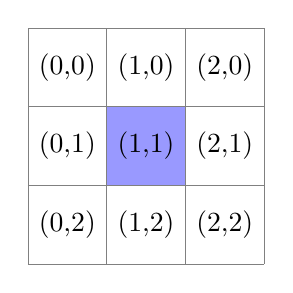
\begin{tikzpicture}
\draw[step=1cm,gray,very thin] (-2,-2) grid (1,1);
\fill[blue!40!white] (0,0) rectangle (-1,-1);
\draw (-1.5, +0.5) node {(0,0)};
\draw (-0.5, +0.5) node {(1,0)};
\draw (0.5, +0.5) node {(2,0)};
\draw (-1.5, -0.5) node {(0,1)};
\draw (-0.5, -0.5) node {(1,1)};
\draw (0.5, -0.5) node {(2,1)};
\draw (-1.5, -1.5) node {(0,2)};
\draw (-0.5, -1.5) node {(1,2)};
\draw (0.5, -1.5) node {(2,2)};
\end{tikzpicture}
}

En la figura también aparece el sistema de coordenadas con el que identificaremos cada celda en la ventana gráfica. En particular, al pixel que se encuentra en el centro de la ventana gráfica {\tt (width/2, height/2)} le corresponde la celda (1, 1) o al píxel  {\tt (2*width/3, height/3)}  le corresponde la celda $(2,0)$.  Como dibujaremos celdas en este ejercicio, usaremos la función \cm{rect()} suministrando el vértice más cercano al origen (``el superior izquierdo'') y la longitud del cuadrado. NO se usará otra función para dibujar los cuadrados o celdas.

\noindent Construye las siguientes funciones en cada uno de los siguiente módulos. Presta atención a los enunciados: $(i, j)$ son coordenadas de celdas y $(x, y)$ son coordenadas de pantalla.

{\bf Funciones de relleno:} Todas las funciones, salvo la \cm{rellenaN2Celdas} tiene como parámetro la longitud del lado de las celdas.
\begin{itemize}
\item \cm{rellenaCelda}: Dada una celda $(i, j)$, dibujarla con el color de relleno dado, según el sistema RGB.

\item \cm{rellenaPosicion}: Dada una coordenada $(x, y)$ de la pantalla, dibujar la celda $(i, j)$ que le corresponda con un color de relleno dado, según el sistema RGB. Invoca a la función \cm{rellenaCelda}.

\item \cm{rellenaPosicionRnd}: Dada una coordenada $(x, y)$ de la pantalla, dibujar la celda $(i, j)$ que le corresponda con color de relleno aleatorio, según el sistema RGB.  Invoca a la función \cm{rellenaPosicion}.

\item \cm{rellenaN2Celdas}: Invocando a la función \cm{rellenaPosicionRnd}, dibuja $n^2$ cuadrados (no necesariamente distintos) para valores $(x, y)$ aleatorios, con $n$ el número de particiones que se hacen de los lados de la ventana gráfica cuadrada.
\end{itemize}


{\bf Funciones de dibujo:} Todas las funciones tiene como parámetro el número de celdas en los que se dividen los lados de la ventana gráfica (en el dibujo es 3).
\begin{itemize}
\item \cm{dibujaAdyacentes}: Escribe una función, para la que dada una celda $(i,j)$ dibuja las 4 celdas adyacentes (arriba, abajo, izquierda y derecha) con un color dado.
	Invoca a \cm{rellenaCelda}.
	
	\begin{itemize} 
	\item Esta función tendrá varias líneas de código, pero {\bf solo una linea} contendrá la función \cm{rellenaCelda()}.
	\item Esta función no invocará a  \cm{rellenaCelda()} para celdas inexistentes. 
	
	Por ejemplo, si se invoca a esta función, \cm{dibujaAdyacentes}, para la celda (0,0) no se puede invocar a \cm{rellenaCelda()} para los adyacentes (-1, 0) y (0,-1) porque simplemente no existen.
	\end{itemize}
	
		
\item \cm{dibujaContorno}. Escribe la función para la que dada una coordenada de la pantalla $(x, y)$ y dado un color dibuje las 4 celdas adyacentes a la celda que le corresponde a dicho píxel invocando a \cm{dibujaAdyacentes} para el color suministrado, y rellena la celda que le corresponde al píxel o bien en color blanco o o bien en negro (aleatoriamente) invocando a \cm{rellenaPosicion}.

\item \cm{dibuja}. Invoca a la función anterior después de este proceso.

Dado el pixel  $(x,y)$, obtener  la intensidad de color de los 3 canales, $(r, g,b)$, y generar un número aleatorio entre 0 y 100, que representa una probabilidad.
Entonces, con un 60\% generar nuevos colores  $(r, g,b)$ aleatorios, con un 30\% duplicar los valores $(r, g,b)$ y con otro 10\% quedarse con la mitad de dos dichos valores.

	Las instrucciones {\tt red(get(x, y))}, {\tt green(get(x, y))} y {\tt blue(get(x, y))} permiten obtener la intesidad RGB. Así invocadas retornan valores entre 0 y 255.
	
\item \cm{dibujaKCeldas}. Construye una función que invoca a la anterior para $K$-coordenadas $(x, y)$ aleatorias.

\end{itemize}

{\bf Función de inicio}
\begin{itemize}
\item \cm{solucion}. Construye una última función que pida al usuario 2 valores: el número de cuadrados a dibujar inicialmente (el $n$ para dibujar $n^2$ cuadrados) y el valor $K$ de la  la última función (para modificar $K$ cuadrados).

Para comprobar el funcionamiento de tu programa puedes usar la instrucción \cm{save()} dos veces: una para guardar la imagen antes de modificar K=1 cuadrado y la imagen después de haber modificado $K=1$ cuadrado.
\end{itemize}

Invoca a \cm{solucion} desde la función principal y construye los módulos pertinentes.

Opcionalmente, haz una versión interactiva para que el valor $(x, y)$ se corresponda con {\tt (mouseX, mouseY)} cuando el usuario haga click,


% - - - - - - - - - - - - - - - - - - - - - - - - - - - - - - - - - - - - - - - - - - - -

\input ejercicios/05-Funciones/DibujaAdyacentesSol.tex


%%%%%%%%%%%%%%%%%%%%%%%%%%%%%%%%%%%%%%%%%%%%%%%%%% 
%
%
%\item \nivel{3}
%
%Escribe un programa que incluya lo siguiente:
%\begin{itemize}
%	\item Una función que determine si un número natural es primo o no.
%	\item Una función que determine si un número natural es un número de Mersenne o no. Se dice que un número n es un número de Mersenne si es una unidad menor que una potencia de 2.
%	\item Una función que determine si un número es un primo de Mersenne, para lo cual debe cumplir al mismo tiempo que sea un número primo y que sea un número de Mersenne.
%	\item Una función que permita conocer la cantidad de números primos de Marsenne en un rango de valores [a,b].
%	\item Un programa principal que solicite dos valores naturales al usuario y determine la cantidad números primos de Marsenne en el rango que constituyen esos dos valores.
%\end{itemize}
%
%Cada función debe de invocar a la anterior. El programa principal debe de invocar igualmente a la última de las funciones. \\
%
%


%%%%%%%%%%%%%%%%%%%%%%%%%%%%%%%%%%%%%%%%%%%%%%%%%% 
\separacion
\subsection{Codificación de fechas}
\objetivo{3}{-}{Construcción de un programa modular. Resolución de problemas.}

Se opta por codificar la fecha y hora por números naturales no inferiores a 11 cifras de acuerdo a este esquema:

$$
\underbrace{aaaa}_{\mbox{\small \it año}}
\overbrace{mm}^{mes}
\underbrace{dd}_{\mbox{\small \it día}}
\overbrace{hh}^{hora}
\underbrace{nn}_{minutos}
\overbrace{ss}^{segundos}
$$
Por ejemplo,  10101000001 representa el primer segundo del primer dia del año 1 y 20180920233005 representa a la hora 23h 30' 5'' del día 20 de septiembre (mes 9) de 2018.

Haz un programa que las siguientes funciones:

\begin{itemize}
\item Dado un número $n$ comprobar que es un número válido. Se asumen que todos los meses de febrero tienen 28 días (no hay años bisiestos).

P.e.: el número 1000230569001 no es válido porque tendría esta descomposición
$$
\underbrace{100}_{\mbox{\small \it año}}
\overbrace{02}^{mes}
\underbrace{30}_{\mbox{\small \it día}}
\overbrace{56}^{hora}
\underbrace{90}_{minutos}
\overbrace{01}^{segundos}
$$
y claramente no existen horas con 90 minutos, ni tenemos días de 56 horas, y el mes de febrero no tiene 30 días.

\

Construye para cada dato dos funciones: la que extrae la información y la que comprueba que la información es correcta. 
Por ejemplo, para los minutos implementa la función que obtiene los minutos y la que comprueba si esos minutos son válidos.
Observa que las que obtienen los datos deberían a su vez invocar a una función que ``extrae'' las cifras adecuadas (para sus distintos argumentos).


\item Dado un número $n$, construye las 5 funciones que incrementan en una unidad cada una de las componentes generando números válidos.

P.e. la función que incrementa en una unidad los segundos aplicada al número 20181231235959 que representa al último segundo del año 2018
retornaría el número 20190101000000 que se corresponde que el instante inicial del primer día del año 2019. Notar que la función que
incrementa en un 1 segundo puede invocar a la que incrementa en un 1 minuto, y ésta a la que incrementa en 1 hora, y así sucesivamente.

\item Crea tu propio reloj en la ventana gráfica usando la función \cm{draw()} incrementando 1 segundo en cada ciclo. Usa estas funciones.

\begin{itemize}
\item Dado un número $n$ mostrar su hora en el centro de la ventana gráfica como si fuera un reloj digital. Por ejemplo para el número 20180920233005 se mostraría 23:30:05
\item Dado un número $n$ mostrar en la parte superior de la ventana gráfica la fecha en letra. Por ejemplo para el número 20180920233005 se mostraría ``2 de septiembre de 2018''.
\item Las equivalentes que muestran la información en la consola.
\end{itemize}

\item Crea dos módulos. Uno con las funciones que manipulan fechas codificadas y otro con las funciones que muestran la fecha descodificada.
\end{itemize}

Una versión simplificada de este ejercicio es considerar que se trabaja únicamente con número de 6 cifras que codifican la hora: ``hh:mm:ss''.  Para demostrar que sabe realizar el ejercicio desarrolle primero esta versión simplificada. Extienda con posterioridad a la versión completa con números de al menos 11 cifras: ``año:mes:dia:hh:mm:ss''.


% - - - - - - - - - - - - - - - - - - - - - - - - - - - - - - - - - - - - - - - - - - - -

\input ejercicios/05-Funciones/CodificacionHorariaSol.tex


%%%%%%%%%%%%%%%%%%%%%%%%%%%%%%%%%%%%%%%%%%%%%%%%%% 

%\item \nivel{3} 

%Cada partida de whitejack se juega con varios mazos de la baraja inglesa. 
%
%El valor de las cartas es:
%\parbox{.75\textwidth}{
%\begin{tabular}{|l|ccccc|} \hline
%Carta & As & K & Q & J & 10-2 \\ 
%Valor & 1 o 11 & 2 o 10 &  3 o 9 & 4 o 8 & Su número \\ \hline
%\end{tabular}
%}
%
%El valor final desde la J hasta el As  lo decide el jugador cuando la mesa le entregue la carta.
%
%Inicialmente  la mesa  entrega una carta al jugador.
%Si el jugador decide seguir jugando tiene que indicar cuántas cartas quiere que le entreguen.
%Si la suma de los puntos de las cartas supera el 51 pierde el jugador,  y en otro caso pierde.
%
%Haga un programa que realice una partida de whitejack indicando si el jugador gana o pierde.
%Las cartas se generarán de forma aleatoria con naturales mediante funciones \texttt{dameNumero} y \texttt{damePalo}.
%Diseña también la función \texttt{muestraCarta}  que imprime un mensaje indicado al jugador qué carta se le ha dado, en función de dos números naturales según la tablas siguientes, y los puntos que lleva acumulados antes de que le entregaran esa carta.
%\begin{center}
%\begin{tabular}{|l|ccccc|} \hline
%Valor del Número & 1 & 13 & 12 & 11 & 10-2 \\ 
%Texto a mostrar & As & Rey (K) &  Reina (Q) & Caballero (J) & El número \\ \hline
%\end{tabular}\\
%\begin{tabular}{|l|cccc|} \hline
%Valor del Palo & 0 & 1 & 2 & 3 \\ 
%Texto a mostrar & Tréboles & Corazones &  Rombos & Picas \\ \hline
%\end{tabular}
%\end{center}


%%%%%%%%%%%%%%%%%%%%%%%%%%%%%%%%%%%%%%%%%%%%%%%%%% 

\separacion